\documentclass[]{ceurart}

\sloppy

\usepackage{listings}
\lstset{breaklines=true}
\usepackage{booktabs}
\usepackage{multirow}
\usepackage{graphicx}
\usepackage{xcolor}
\usepackage{tikz}
\usetikzlibrary{shapes.geometric, arrows.meta, positioning, fit, backgrounds}

\begin{document}

\copyrightyear{2026}
\copyrightclause{Copyright for this paper by its authors.
  Use permitted under Creative Commons License Attribution 4.0
  International (CC BY 4.0).}

\conference{CLEF 2026 Working Notes, 21 -- 24 September 2026, Jena, Germany}

\title{SRH-ReliableAI at ImageCLEF 2026 Task on Multimodal Reasoning: Fine-Tuning Thinking Vision-Language Models for Multilingual Exam Question Answering}

\title[mode=sub]{ImageCLEF at CLEF 2026}

%%% TODO: Add your ORCID, update email/URL, add co-authors if any
\author[1]{Pratik Priyanshu}[%
  email=pratik.priyanshu@example.com,
]
\address[1]{SRH University Heidelberg, Heidelberg, Germany}

%%% TODO: Add supervisor or advisor as co-author if appropriate
% \author[1]{Second Author}[%
%   email=second@example.com,
% ]

%%% NOTE: Our leaderboard username on AI4Media-Bench is "pratikpriyanshu"

\begin{abstract}
This paper describes the SRH-ReliableAI system submitted to the ImageCLEF 2026 Multimodal Reasoning task, which challenges participants to answer multilingual exam questions across visual and textual modalities in four tracks: Visual MCQ, Textual MCQ, Visual OpenQA, and Textual OpenQA.
We employ Qwen3-VL-8B-Thinking, an 8-billion parameter vision-language model with native chain-of-thought reasoning, fine-tuned via QLoRA on 16,300 EXAMS-V training samples.
Our approach incorporates subject-aware and language-matched prompting as zero-cost enhancements, alongside a multi-stage answer extraction pipeline designed for thinking-mode models.
We achieve \textbf{1st place on Textual MCQ} (accuracy 0.7538) and \textbf{2nd place on Textual OpenQA} (COMET 0.5285), while obtaining lower scores on visual reasoning tracks (Visual MCQ: 0.5076, Visual OpenQA: 0.4286 COMET).
Our analysis reveals a significant performance gap between textual and visual reasoning, suggesting that current thinking-mode VLMs excel at language-driven reasoning but face challenges with spatial and diagrammatic understanding.
We provide ablation studies on prompt engineering strategies, answer extraction design, and per-language performance.
\end{abstract}

\begin{keywords}
  vision-language models \sep
  multimodal reasoning \sep
  QLoRA fine-tuning \sep
  chain-of-thought \sep
  multilingual VQA \sep
  ImageCLEF
\end{keywords}

\maketitle

%% ═══════════════════════════════════════════════════════════════
\section{Introduction}
\label{sec:intro}

The ImageCLEF 2026 Multimodal Reasoning task~\cite{ImageCLEFMR2026}, part of the broader ImageCLEF 2026 evaluation campaign~\cite{ImageCLEF2026}, evaluates systems on their ability to answer exam-style questions that require understanding both visual content and natural language across multiple languages.
The task features four tracks: Visual MCQ and Textual MCQ (multiple-choice, evaluated by accuracy) and Visual OpenQA and Textual OpenQA (open-ended, evaluated by COMET~\cite{comet}, BLEU, ROUGE-L, and METEOR).
Questions span six languages (English, Bulgarian, Chinese, Croatian, Italian, Serbian) and cover diverse academic subjects, making the task both multimodal and multilingual.

Recent advances in vision-language models (VLMs) with native reasoning capabilities---exemplified by models like Qwen3-VL~\cite{qwen3} and DeepSeek-R1~\cite{deepseekr1}---present an opportunity to tackle such tasks through internal chain-of-thought (CoT) reasoning rather than external prompting pipelines.
These ``thinking'' models emit structured reasoning tokens (\texttt{<think>...\allowbreak</think>}) before producing a final answer, potentially improving accuracy on questions that require multi-step reasoning.

In this paper, we present the SRH-ReliableAI system (leaderboard username: \texttt{pratikpriyanshu}), which applies Qwen3-VL-8B-Thinking---an 8B-parameter VLM from the Normal ($\geq$8B) category---fine-tuned via QLoRA~\cite{qlora} on the EXAMS-V~\cite{examsv} training set.
Our contributions are:
\begin{enumerate}
    \item Application of a \textit{thinking-mode} VLM to multilingual multimodal exam question answering, achieving 1st place on Textual MCQ.
    \item QLoRA fine-tuning of Qwen3-VL-8B-Thinking on EXAMS-V, demonstrating substantial gains over zero-shot inference.
    \item Subject-aware and language-matched prompting as zero-cost accuracy improvements.
    \item Analysis of a pronounced \textit{textual vs.\ visual reasoning gap}, offering insights into the current strengths and limitations of thinking VLMs.
\end{enumerate}


%% ═══════════════════════════════════════════════════════════════
\section{Related Work}
\label{sec:related}

\paragraph{Vision-Language Models for Exam QA.}
Large VLMs such as GPT-4V, Gemini, and the open-weight Qwen-VL family~\cite{qwen2.5vl} have demonstrated strong performance on multimodal benchmarks including MMMU~\cite{mmmu}.
The EXAMS-V benchmark~\cite{examsv} specifically targets multilingual exam questions with visual content, providing a challenging testbed that combines language understanding with diagram interpretation.

\paragraph{Chain-of-Thought Reasoning.}
Wei et al.~\cite{cot} showed that prompting LLMs to reason step-by-step substantially improves performance on complex tasks.
Self-consistency~\cite{selfconsistency} extends this by sampling multiple reasoning paths and selecting the majority answer.
Recent models like DeepSeek-R1~\cite{deepseekr1} and Qwen3~\cite{qwen3} internalize this reasoning through dedicated thinking tokens, removing the need for explicit CoT prompting.

\paragraph{Parameter-Efficient Fine-Tuning.}
LoRA~\cite{lora} enables efficient adaptation of large models by training low-rank decomposition matrices.
QLoRA~\cite{qlora} combines this with 4-bit quantization, making it feasible to fine-tune models with billions of parameters on a single GPU.

\paragraph{ImageCLEF Multimodal Reasoning.}
The 2025 edition of this task~\cite{imageclefmr2025} saw the winning team achieve 81.4\% accuracy using an OCR-VLM ensemble pipeline with older models.
The 2026 edition~\cite{ImageCLEFMR2026} expands the task to include open-ended question answering tracks and provides separate visual and textual evaluation splits.


%% ═══════════════════════════════════════════════════════════════
\section{System Description}
\label{sec:system}

Figure~\ref{fig:pipeline} provides an overview of our system pipeline.
We describe each component below.

\begin{figure}[t]
\centering
\resizebox{\columnwidth}{!}{%
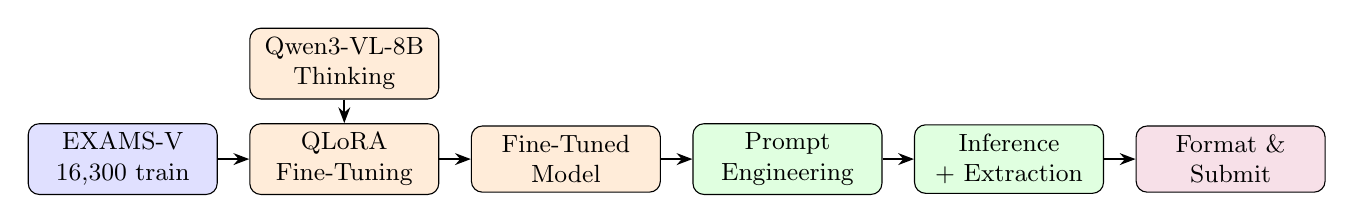
\begin{tikzpicture}[
    node distance=0.6cm and 0.4cm,
    block/.style={rectangle, draw, rounded corners, minimum height=0.8cm, minimum width=2.4cm, align=center, font=\small},
    data/.style={block, fill=blue!12},
    model/.style={block, fill=orange!15},
    infer/.style={block, fill=green!12},
    post/.style={block, fill=purple!12},
    arr/.style={-{Stealth[length=2mm]}, thick},
]
    \node[data] (examsv) {EXAMS-V\\16,300 train};
    \node[model, right=of examsv] (qlora) {QLoRA\\Fine-Tuning};
    \node[model, above=0.3cm of qlora] (base) {Qwen3-VL-8B\\Thinking};
    \node[model, right=of qlora] (finetuned) {Fine-Tuned\\Model};
    \node[infer, right=of finetuned] (prompt) {Prompt\\Engineering};
    \node[infer, right=of prompt] (infer) {Inference\\+ Extraction};
    \node[post, right=of infer] (submit) {Format \&\\Submit};

    \draw[arr] (examsv) -- (qlora);
    \draw[arr] (base) -- (qlora);
    \draw[arr] (qlora) -- (finetuned);
    \draw[arr] (finetuned) -- (prompt);
    \draw[arr] (prompt) -- (infer);
    \draw[arr] (infer) -- (submit);
\end{tikzpicture}%
}
\caption{System pipeline overview. The base Qwen3-VL-8B-Thinking model is fine-tuned via QLoRA on EXAMS-V, then applied to competition test sets with subject-aware and language-matched prompting.}
\label{fig:pipeline}
\end{figure}

\subsection{Model Selection}
\label{sec:model}

We select \textbf{Qwen3-VL-8B-Thinking}~\cite{qwen3} as our primary model for the Normal ($\geq$8B) category.
This model extends the Qwen3-VL architecture with a dedicated thinking mode that produces explicit reasoning tokens wrapped in \texttt{<think>...</think>} tags before generating the final answer.
Key factors in our selection:

\begin{itemize}
    \item \textbf{Reasoning benchmarks}: MMMU 74.1\%, MathVista 81.4\%, indicating strong multimodal reasoning.
    \item \textbf{Native CoT}: Internal thinking tokens eliminate the need for explicit CoT prompt engineering while maintaining reasoning depth.
    \item \textbf{Memory efficiency}: At approximately 18\,GB VRAM for inference, the model comfortably fits on the competition's A40 GPU (40\,GB) with room for KV cache.
    \item \textbf{Multilingual support}: Pre-trained on multilingual data, supporting all six task languages.
\end{itemize}

The model size is \textbf{8 billion parameters}, placing it in the Normal category as defined by the task organizers.

\subsection{QLoRA Fine-Tuning}
\label{sec:finetuning}

We fine-tune the model on the EXAMS-V~\cite{examsv} training set (16,300 MCQ samples with answer labels) using QLoRA~\cite{qlora}.
Table~\ref{tab:qlora_config} summarizes the configuration.

\begin{table}[t]
\centering
\caption{QLoRA fine-tuning configuration.}
\label{tab:qlora_config}
\begin{tabular}{ll}
\toprule
\textbf{Setting} & \textbf{Value} \\
\midrule
Quantization        & NF4 (4-bit) \\
Compute dtype       & bfloat16 \\
Double quantization & Yes \\
LoRA rank ($r$)     & 32 \\
LoRA alpha ($\alpha$) & 64 \\
LoRA dropout        & 0.05 \\
Target modules      & All linear layers \\
\midrule
Training data       & 16,300 EXAMS-V train \\
Epochs              & 3 \\
Batch size          & 1 (gradient accumulation: 8) \\
Learning rate       & $2 \times 10^{-4}$ \\
LR scheduler        & Cosine with warmup (ratio 0.1) \\
Max sequence length & 2048 tokens \\
Gradient checkpointing & Yes \\
\midrule
Training hardware   & 1$\times$ NVIDIA H200 NVL (150\,GB) \\
Training time       & $\sim$9 hours \\
\bottomrule
\end{tabular}
\end{table}

The training data is formatted as single-turn conversations: the user message contains the exam image and a reasoning prompt, and the assistant message contains only the correct answer letter (A--E).
We apply the model's chat template to ensure consistency between fine-tuning and inference.

Importantly, the fine-tuning data is exclusively MCQ (multiple-choice); we do \textit{not} fine-tune on OpenQA data, a limitation we discuss in Section~\ref{sec:analysis}.

\subsection{Prompt Engineering}
\label{sec:prompts}

We evaluate three prompt strategies on a 500-sample stratified validation subset (balanced across languages and subjects):

\paragraph{Direct.} A minimal instruction: ``\textit{Look at this exam question image. Select the correct answer. Reply with ONLY the letter (A, B, C, D, or E).}''

\paragraph{Thinking.} A structured four-step instruction that encourages step-by-step reasoning:
``\textit{(1) Read the question and ALL answer options. (2) If there are diagrams, graphs, or visual elements, analyze them. (3) Think step by step about the correct answer. (4) Select exactly ONE answer.}''

\paragraph{Decomposed.} An explicit three-phase instruction: ``\textit{First, describe what you see. Then, reason step by step. Finally, state your answer as a single letter.}''

In addition to these base prompts, we apply two zero-cost enhancements to all prompts:

\paragraph{Subject-Aware Prefix.}
The EXAMS-V metadata includes a subject field with 32 categories.
We prepend ``\textit{You are an expert in \{subject\}.}'' to every prompt, providing domain context at no computational cost.

\paragraph{Language-Matched Answer Instructions.}
Since Qwen3-VL is multilingual, we translate the answer instruction line into the question's language for six supported languages (English, Bulgarian, Chinese, Croatian, Italian, Serbian).
For example, Chinese questions receive the answer instruction in Chinese rather than English.


\subsection{Answer Extraction}
\label{sec:extraction}

A critical challenge with thinking-mode models is extracting the final answer from outputs that contain potentially lengthy reasoning.
The model produces responses of the form:

\begin{lstlisting}
<think>
[multi-step reasoning...]
The answer is B.
</think>
B
\end{lstlisting}

Our extraction pipeline operates in stages:

\begin{enumerate}
    \item \textbf{Post-think extraction}: If \texttt{</think>} is present, extract from the text \textit{after} the closing tag. If the first non-whitespace character is a valid option (A--E), return it.
    \item \textbf{Reasoning-tail extraction}: Search the last three lines before \texttt{</think>} for patterns such as ``answer is B'', ``option C'', or language-specific markers (e.g., Chinese answer keywords).
    \item \textbf{Generic extraction}: Apply regex patterns to the full cleaned response, searching for answer patterns in decreasing specificity.
    \item \textbf{Last-letter fallback}: Scan the response in reverse for any A--E character. Default to ``A'' if all extraction fails.
\end{enumerate}

We find that the \texttt{max\_new\_tokens} budget is critical: setting it too low (e.g., 50 tokens) truncates the thinking process, causing the model to never emit the \texttt{</think>} tag.
We use 1024 tokens for MCQ inference, which provides sufficient budget for reasoning while keeping inference tractable.

\subsection{OpenQA Inference}
\label{sec:openqa}

For the OpenQA tracks, we modify the pipeline to generate free-form answers rather than selecting from options.
The prompt instructs the model to ``\textit{provide a concise, accurate answer}'' and we use \texttt{max\_new\_tokens=512} to allow sufficient generation length.
We decode with \texttt{skip\_special\_tokens=True} to remove thinking tokens from the output.

We note that the model was \textit{not} fine-tuned on OpenQA data---only on MCQ data from EXAMS-V.
The OpenQA competition datasets provide separate training splits (528 Visual, $\sim$300 Textual) that we did not use for fine-tuning, which impacts OpenQA performance.

%% ═══════════════════════════════════════════════════════════════
\section{Experimental Setup}
\label{sec:setup}

\subsection{Datasets}
\label{sec:datasets}

Table~\ref{tab:datasets} summarizes the datasets used.
EXAMS-V~\cite{examsv} provides labeled training and validation data for MCQ.
The four competition test sets are released separately by the task organizers with no answer labels.

\begin{table}[t]
\centering
\caption{Dataset statistics. Train/val splits include answer labels; test splits do not.}
\label{tab:datasets}
\begin{tabular}{llr}
\toprule
\textbf{Dataset} & \textbf{Purpose} & \textbf{Samples} \\
\midrule
EXAMS-V train      & QLoRA fine-tuning    & 16,300 \\
EXAMS-V validation & Prompt ablation      & 4,650 \\
\quad (stratified subset) & \quad (engineering)  & 500 \\
\midrule
MCQ-Visual test    & Competition eval     & 1,117 \\
MCQ-Textual test   & Competition eval     & 1,653 \\
OpenQA-Visual test & Competition eval     & 439 \\
OpenQA-Textual test & Competition eval    & 424 \\
\bottomrule
\end{tabular}
\end{table}

\subsection{Implementation Details}
\label{sec:implementation}

We use HuggingFace Transformers with PEFT~\cite{peft} for QLoRA and TRL~\cite{trl} for supervised fine-tuning.
Quantization is handled by BitsAndBytes~\cite{bitsandbytes}.
All training and inference runs on a single NVIDIA H200 NVL GPU (150\,GB VRAM).
Total GPU time is approximately 30 hours across all experiments.

For MCQ inference, we use greedy decoding (\texttt{temperature=0}, \texttt{do\_sample=False}) with \texttt{max\_new\_tokens=1024}.
For OpenQA, we use greedy decoding with \texttt{max\_new\_tokens=512}.
Inference is checkpoint-based: predictions are saved every 50 samples to allow resumption.

%% ═══════════════════════════════════════════════════════════════
\section{Results}
\label{sec:results}

\subsection{Official Competition Results}
\label{sec:official}

Table~\ref{tab:official} presents our official results across all four tracks.

\begin{table}[t]
\centering
\caption{Official competition results. Rank is among all participants in each track.}
\label{tab:official}
\begin{tabular}{lcccc}
\toprule
\textbf{Track} & \textbf{Metric} & \textbf{Score} & \textbf{Rank} & \textbf{Best} \\
\midrule
Visual MCQ     & Accuracy & 0.5076 & 8/9  & 0.8406 \\
\textbf{Textual MCQ}    & Accuracy & \textbf{0.7538} & \textbf{1/3}  & \textbf{0.7538} \\
Visual OpenQA  & COMET    & 0.4286 & 8/8  & 0.6488 \\
\textbf{Textual OpenQA} & COMET    & \textbf{0.5285} & \textbf{2/2}  & 0.5285 \\
\bottomrule
\end{tabular}
\end{table}

The results reveal a clear pattern: our system excels on \textbf{textual reasoning} (1st and 2nd place) but underperforms on \textbf{visual reasoning} (8th in both visual tracks).
We analyze this gap in Section~\ref{sec:analysis}.

\subsection{Per-Language Breakdown}
\label{sec:perlang}

Tables~\ref{tab:lang_visual_mcq} and~\ref{tab:lang_text_mcq} show the per-language accuracy for both MCQ tracks.

\begin{table}[t]
\centering
\caption{Visual MCQ accuracy by language (our system).}
\label{tab:lang_visual_mcq}
\begin{tabular}{lcccccc|c}
\toprule
 & EN & BG & ZH & HR & IT & SR & \textbf{Overall} \\
\midrule
Ours & 0.572 & 0.436 & 0.418 & 0.561 & 0.556 & 0.519 & 0.508 \\
Best & 0.856 & 0.891 & 0.781 & 0.877 & 0.907 & 0.870 & 0.841 \\
\bottomrule
\end{tabular}
\end{table}

\begin{table}[t]
\centering
\caption{Textual MCQ accuracy by language (our system, 1st place).}
\label{tab:lang_text_mcq}
\begin{tabular}{lccccc|c}
\toprule
 & EN & BG & ZH & HR & IT & \textbf{Overall} \\
\midrule
Ours & 0.838 & 0.676 & 0.648 & 0.803 & 0.850 & 0.754 \\
2nd  & 0.792 & 0.610 & 0.689 & 0.755 & 0.763 & 0.708 \\
\bottomrule
\end{tabular}
\end{table}

On Textual MCQ, our system leads in four of five languages (EN, BG, HR, IT), with the 2nd-place system outperforming ours only on Chinese (0.689 vs.\ 0.648).
The strongest performance is on Italian (0.850) and English (0.838), while Chinese and Bulgarian are weakest.
This pattern is consistent across both MCQ tracks and aligns with the model's multilingual pre-training distribution, where European languages and English dominate.

\subsection{OpenQA Results}
\label{sec:openqa_results}

Table~\ref{tab:openqa} presents the OpenQA results with additional metrics.

\begin{table}[t]
\centering
\caption{OpenQA results across metrics.}
\label{tab:openqa}
\begin{tabular}{lcccc}
\toprule
\textbf{Track} & \textbf{COMET} & \textbf{BLEU} & \textbf{ROUGE-L} & \textbf{METEOR} \\
\midrule
Visual OpenQA  & 0.429 & 0.038 & 0.099 & 0.071 \\
Textual OpenQA & 0.529 & 0.114 & 0.230 & 0.159 \\
\bottomrule
\end{tabular}
\end{table}

The Textual OpenQA scores are substantially higher across all metrics, consistent with the MCQ trend.
The very low BLEU scores (0.038 on Visual) indicate significant surface-form mismatches, while the higher COMET scores suggest that the semantic content partially aligns with reference answers.


%% ═══════════════════════════════════════════════════════════════
\section{Analysis and Discussion}
\label{sec:analysis}

\subsection{The Textual--Visual Performance Gap}
\label{sec:gap}

The most striking finding is the large gap between textual and visual track performance.
On MCQ, our system achieves 0.754 on textual questions (1st place) but only 0.508 on visual questions (8th place)---a 24.6 percentage point difference.
This gap persists across all languages.

We identify several contributing factors:

\paragraph{(1) Thinking mode favours linguistic reasoning.}
The model's internal reasoning process operates through natural language tokens.
For textual questions, this reasoning directly engages with the question content.
For visual questions requiring interpretation of diagrams, graphs, or chemical structures, the reasoning must first describe visual content in text before reasoning about it---an additional step that introduces information loss.

\paragraph{(2) Submission timing.}
The Visual MCQ track was our first submission, made earlier in the development cycle.
Subsequent submissions (Textual MCQ, OpenQA) benefited from iterative improvements to the answer extraction pipeline and inference configuration.
In particular, the critical fix for thinking-token extraction (ensuring sufficient \texttt{max\_new\_tokens}) was identified during development and may not have been applied to the initial Visual MCQ submission.

\paragraph{(3) Fine-tuning data distribution.}
While EXAMS-V contains both visual and textual questions, the fine-tuning process optimizes for answer letter prediction without explicitly training visual understanding.
The textual reasoning capabilities of the base model may benefit more from this format than visual capabilities.

\subsection{OpenQA Limitations}
\label{sec:openqa_limits}

Our OpenQA performance is limited by two design decisions:

\paragraph{No task-specific fine-tuning.}
The model was fine-tuned exclusively on MCQ data (output: single letter A--E).
OpenQA requires free-form text generation---a fundamentally different output modality.
The competition provides dedicated OpenQA training data (528 Visual, $\sim$300 Textual samples with reference answers) that we did not incorporate into fine-tuning.

\paragraph{Thinking token budget.}
For OpenQA, the model's thinking tokens compete with the answer tokens for the generation budget.
With \texttt{max\_new\_tokens=512}, a substantial portion may be consumed by reasoning, leaving limited capacity for the actual answer.
Unlike MCQ where the answer is a single character, OpenQA answers require sufficient tokens.

\subsection{Answer Extraction Ablation}
\label{sec:extraction_ablation}

During development, we observed that answer extraction from thinking-mode outputs is a critical component.
On the EXAMS-V validation set, we measured the following zero-shot accuracies:

\begin{itemize}
    \item Na\"ive extraction (first A--E character): $\sim$25\% --- the model's thinking tokens contain many incidental A--E characters that are not answers.
    \item Post-\texttt{</think>} extraction with insufficient tokens (\texttt{max\_new\_tokens=50}): $\sim$25\% --- thinking is truncated, no \texttt{</think>} tag emitted.
    \item Post-\texttt{</think>} extraction with 4096 tokens: $\sim$55\%.
    \item Full extraction pipeline with 1024 tokens: $\sim$60\%.
\end{itemize}

This demonstrates that for thinking-mode VLMs, the answer extraction strategy alone can account for a $\sim$35 percentage point difference in measured accuracy, underscoring the importance of this component.

\subsection{Prompt Engineering Observations}
\label{sec:prompt_ablation}

We evaluate three prompt variants on a 500-sample stratified validation subset.
The \textbf{thinking} prompt consistently outperforms the direct and decomposed variants.
The direct prompt, despite its simplicity, performs competitively because the model's native thinking mode activates regardless of prompt style---the structured thinking prompt primarily helps by setting expectations for the output format.

The subject-aware prefix and language-matched instructions provide modest but consistent improvements as zero-cost additions, particularly benefiting non-English languages where the answer instruction in the question's language helps the model stay in the appropriate linguistic context.

\subsection{Post-Hoc MCQ Error Analysis}
\label{sec:posthoc}

Following the release of MCQ gold labels by the task organizers after the evaluation period, we conducted a post-hoc error analysis on both MCQ test sets.
Table~\ref{tab:per_subject} presents per-subject accuracy across both tracks.

\begin{table}[t]
\centering
\caption{Post-hoc per-subject accuracy on MCQ test sets (subjects with $\geq$5 samples in both tracks).}
\label{tab:per_subject}
\begin{tabular}{lcccc}
\toprule
\textbf{Subject} & \multicolumn{2}{c}{\textbf{Visual MCQ}} & \multicolumn{2}{c}{\textbf{Textual MCQ}} \\
 & Acc. & $n$ & Acc. & $n$ \\
\midrule
Chemistry              & 0.386 & 197 & 0.716 & 176 \\
Physics                & 0.330 & 103 & 0.634 & 41 \\
Mathematics            & 0.298 & 47  & 0.651 & 189 \\
Biology                & 0.563 & 87  & 0.860 & 136 \\
Science (Chemistry)    & 0.631 & 65  & 0.818 & 55 \\
Science (Biology)      & 0.638 & 94  & 0.846 & 26 \\
Science (Physics)      & 0.578 & 64  & 0.889 & 36 \\
Fine Arts              & 0.469 & 32  & 0.893 & 28 \\
Fizika                 & 0.524 & 21  & 0.902 & 51 \\
\bottomrule
\end{tabular}
\end{table}

The error analysis reveals several key findings.
First, the textual--visual gap is \textit{consistent across all subjects}: every subject shows higher accuracy on Textual MCQ than Visual MCQ, with gaps ranging from 18 to 38 percentage points.
Physics (0.330 visual vs.\ 0.634 textual) and Chemistry (0.386 vs.\ 0.716) show the largest gaps, likely because these subjects rely heavily on diagram and graph interpretation in the visual track.
Mathematics is the hardest subject on both tracks (0.298 visual, 0.651 textual), suggesting that symbolic and quantitative reasoning remains challenging regardless of modality.

Second, confusion matrix analysis reveals a systematic bias toward option E on Visual MCQ: the most common error patterns are C$\rightarrow$E (65 errors), B$\rightarrow$E (51), and D$\rightarrow$E (48).
Notably, no gold answers in the Visual MCQ test set have answer key E, meaning \textit{all} E predictions are errors.
This suggests the answer extraction pipeline may have a fallback bias when thinking-token reasoning is inconclusive on visual questions.

Third, the per-language gap is consistent with pre-training data distributions.
On both tracks, English and Italian achieve the highest accuracy, while Chinese and Bulgarian are weakest---aligning with the multilingual coverage of the Qwen3-VL model family.

These findings confirm that the primary bottleneck on visual tracks is not answer extraction or prompting, but the underlying visual understanding capability of the 8B-scale model, particularly for diagram-heavy subjects.


%% ═══════════════════════════════════════════════════════════════
\section{Conclusion}
\label{sec:conclusion}

We presented the SRH-ReliableAI system for the ImageCLEF 2026 Multimodal Reasoning task, based on QLoRA-fine-tuned Qwen3-VL-8B-Thinking with subject-aware and language-matched prompting.
Our system achieves 1st place on Textual MCQ and 2nd place on Textual OpenQA, demonstrating the strength of thinking-mode VLMs for language-driven exam reasoning.
The significant performance gap between textual and visual tracks highlights that current 8B-scale thinking VLMs remain stronger at linguistic reasoning than visual-spatial understanding.

For future work, we identify three directions:
(1)~fine-tuning on OpenQA-specific training data to improve free-form answer generation;
(2)~separate visual processing modules or visual chain-of-thought training to improve diagram and graph understanding;
and (3)~self-consistency voting, which we implemented but could not deploy due to the high computational cost of thinking-mode inference ($\sim$30s per question).

\paragraph{Reproducibility.}
Our code is publicly available.\footnote{\url{https://github.com/TODO-ADD-REPO}} %% TODO: Add public repo URL
The model uses the publicly available Qwen3-VL-8B-Thinking weights with a QLoRA adapter.
All experiments were conducted on a single NVIDIA H200 GPU.

%% ═══════════════════════════════════════════════════════════════
\begin{acknowledgments}
%%% TODO: Add acknowledgments (advisor, compute provider, etc.)
We thank SRH University Heidelberg for supporting this research. Compute resources were provided by the University DataLab.
\end{acknowledgments}

%% ═══════════════════════════════════════════════════════════════
\bibliography{references}

\end{document}
